%\newline

%Descripción general del módulo.
%Precondiciones necesarias.
%Por qué existe?
%Qué especificación tiene y cómo se maneja
%Comparación, como manejan los demás trabajos.

\chapter{Diseño}\label{cha:Diseño}

El objetivo principal de este capítulo es describir el diseño del framework propuesto para planificar tareas preemptive en sistemas embebidos heterogéneos. Actualmente existe una gran variedad de planificadores de tareas sobre CPU, la propuesta de esta tesis es presentar el diseño de un framework que ayude a planificar aquellas que se ejecutarán sobre la GPU. El estudio de la planificación de las tareas del CPU está fuera del contexto de esta tesis.
\newline

Aunque se tomó como base el sistema embebido heterogéneo NVIDIA Jetson TX2, el diseño puede ser aplicado a cualquier dispositivo, siempre y cuando cumpla con la característica descritas en la sección \ref{secc:arqPas}.

\section{Descripción general del framework}

La solución propuesta se encuentra dentro de las siguientes clasificaciones:
\begin{itemize}
    \item \textbf{Clasificación por implementación}: \textit{Basado en Software. Partición de Kernel.}
    \item \textbf{Clasificación por planificación}: \textit{Planificación por prioridad.}
    \item \textbf{Clasificación por modificación}: \textit{Modificación de código fuente.}
\end{itemize}

En la Figura \ref{fig:diagramabase} se muestra un diagrama de bloques sobre la arquitectura del framework propuesto. Cada uno de los bloques agrupa las bases necesarias para el funcionamiento del framework.
\newline

El framework está dividido en dos zonas de implementación, la primera tiene que ver con aquellas actividades que son propias del Host, como lo es el protocolo de lanzamiento de los kernel (ver \ref{secc:lanzamientoKernel}. En el caso del manejo de la memoria, debido a que la tarjeta Jetson TX2 utiliza una arquitectura Pascal (ver \ref{secc:arqPas}). Se cuenta con una memoria unificada con lo que se simplifican el manejo de las copias de memoria entre el Host y el Device, resultando en que el módulo \textbf{Memoria} (ver \ref{secc:memoria}) pertenezca a ambas zonas, también se presenta el almacenamiento de los contextos de cada una de las tareas.

En la zona de implementación Device encontramos el módulo \textbf{Puntos Preemptive} ver \ref{secc:puntosPreemptive}). Como su nombre lo indica, se plantea la forma en que el framework implementa las suspensiones y reactivaciones de las tareas una vez alcanzado cada uno de los puntos. 

Un componente fundamental del framework es el módulo \textbf{Planificador} (ver \ref{secc:planificador}), ya que es en donde se dan las pautas para realizar la planificación de las tareas que se ejecutarán en un determinado momento en el Device. Pero para poder realizar dicha prioridad, se plantea el módulo \textbf{Asignación de prioridades}, (ver \ref{secc:asigPrioridad}) el cual se encargará de seleccionar dentro de un conjunto de tareas aquella que tiene la mayor prioridad en un momento específico de tiempo.
\newline

  \begin{figure}[!]
      %\centering
     % \flushleft
        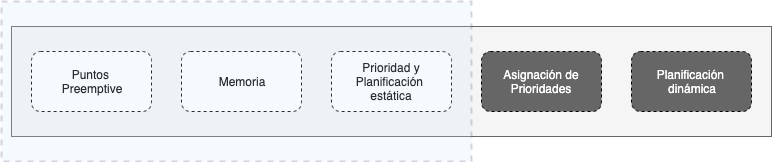
\includegraphics[scale=.6]{diagrama_framework}
        \caption{Esquema del framework para la planificación de tareas preemptive en sistemas embebidos heterogéneos.}
        \label{fig:diagramabase}
    \end{figure}
  
  %Pero en el momento en el que se requiera tener un método de asignación de prioridades personalizado, es necesario tener un módulo que lo permita. Aunado a esto, si por alguna razón se solicita agregar tareas dinámicamente con el sistema en ejecución, se deben tener mecanismos para manejar cualquier interrupción o actualización de información del planificador. Ambos elementos son necesarios en un framework, pero sus componentes internos se dejarán para ser resueltos como trabajo futuro.
  
  %Clasificación y tipo de modificación.

Como se detallará más adelante, esta solución no es transparente al programador, es necesaria la modificación del código fuente. Aunque en un inicio pareciera que el rendimiento es inferior al realizar comprobaciones continuas del estado del quantum, la modificación de las bibliotecas del API o el compilador del dispositivo y la implementación de analizadores sintácticos para la lectura de directivas precompiladas salen de las posibilidades de acción del proyecto, 
por eso no es necesario modificar el código fuente para colocarlas.
\newline 

El diseño del planificador está fuera del contexto de esta tesis, pero se puede implementar con cualquiera en la gama de algoritmos del estado del arte (ver sección \ref{sec:AlgoPlan}).

  \begin{figure}[!]
      \centering
     % \flushleft
        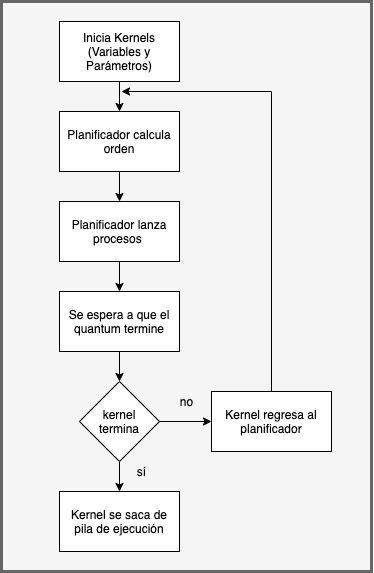
\includegraphics[scale=.58]{flujo}
        \caption{Diagrama del flujo del framework.}
        \label{fig:flujo}
    \end{figure}

\subsection{Precondiciones necesarias} \label{secc:precondiciones}

\begin{itemize}
\item La precondición más importante radica en que el framework debe ser implementado en un programa que funciona correctamente, ya que se realizará una modificación en su código fuente para la implementación del modo preemptive.

\item No se permite la memoria dinámica ni compartida entre kernels.

\item No se permiten apuntadores complejos. 

\item No se permite el llamado a funciones no rastreables.

\item El quantum de las tareas debe ser similar para que aquellas que estén en ejecución terminen en tiempos similares.

\item El número de threads por block debe ser menor o igual a la cantidad de threads disponibles en cada SM.

 \item Los contextos de cada kernel deben poder coexistir en la memoria al mismo tiempo para que se puedan ejecutar y suspender en cada punto preempetive.

\item Todas las tareas que soliciten recursos al planificador deben ser preemptive para que en dado caso puedan ser suspendidas, si así lo requiere el balanceo de carga.

\item Para evitar en la medida de lo posible plazos vencidos, el conjunto de tareas debe ser planificable.

\end{itemize}

\section{Puntos preemptive}\label{secc:puntosPreemptive}

%Descripción general del módulo.

En una aplicación acelerada por el cómputo gráfico muchas veces se implementan más de una función kernel, y en el momento en que ejecutamos varias aplicaciones en la GPU habrá alguna que mantenga en sobretiempo los recursos causando así un retraso en la ejecución en general de todo el sistema.
\newline

Este módulo permite gestionar la actividad de un kernel a nivel de aplicación, aquí se marca la pauta el punto exacto donde se podrá realizar la administración del contexto de una tarea en ejecución, contará con tres casos principales: si se está iniciando el proceso, si está a la mitad de una ejecución o si ya ha terminado, con esto se podrán liberar las unidades de procesamiento para dar lugar a otras tareas de consumir recursos.
\newline

Se propone una serie de puntos de control que se incluirán explícitamente dentro del código que se desea implementar en modo preemptive, esto durante básicamente tres etapas iterativas del ciclo de vida de un kernel a)inicio, b)en ejecución y c)finalización. 
\newline

Este elemento tiene como objetivo que cada que se alcance alguno de los puntos de control dentro de un kernel y sea necesario detener su ejecución, se guarde una copia de su contexto actual en una estructura de datos para que cuando sea nuevamente su oportunidad de ejecución se reanude como si nunca se hubiera detenido. 
\newline

Una vez que una tarea, independientemente del momento de su ciclo de vida en que se encuentre, seguirá ejecutándose en la GPU hasta que complete su cálculo o termine su quantum.
\newline

Al momento de lanzar la tarea siguiente en ejecución se inicializaran todas las variables necesarias en el nuevo contexto por medio de estructura copia de seguridad. Cuando se está en la etapa de inicio de un kernel se inicializan los datos necesarios para el funcionamiento de éste, tanto en su cuerpo, como  en la estructura de datos.
\newline
%Qué especificación tiene y cómo se maneja?

Al inicio del algoritmo \ref{lst:declara} la función kernel está ligeramente modificada en sus parámetros, ya que es necesario que reciba la estructura \textit{Backup} en donde se almacenará su contexto cuando se presente una suspensión preemptive y se recibirá el apuntador al estado del quantum, dicho valor arrojará \textbf{\textit{true}} cuando se haya concluido el tiempo del quantum.
\newline

Como se mencionó anteriormente, esta solución se basa completamente en software, por lo que se debe modificar la función kernel para mantener una convención que ayude a mitigar posibles problemas. Todas las declaraciones de variables deberán realizarse en la primera fase, la cual se encuentra en las primeras líneas del kernel.
\newline

Las únicas declaraciones con inicialización permitidas en esta fase son aquellas que designan la posición tanto de los thread como de los blocks dentro de un grid, esto porque  su información es necesaria en cada una de las siguientes fases. La única variable que es necesaria para todos kernels es \textit{id\_block}, que servirá en las siguientes fases para extraer la información de la estructura \textit{Backup}.

\lstinputlisting[style=CStyle, frame=single,label=lst:declara,  basicstyle=\ttfamily\footnotesize, caption=Fase de declaración de variables.]{algorithms/fase_declaracion.c}

Enseguida pasamos a la fase de la inicialización (ver algoritmo \ref{lst:declara}) de cada una de estas variables y como se muestra en el algoritmo \ref{lst:inicializa} nos apoyamos de una estructura \textit{switch-case} con tres casos dependiendo del estado de cada block. Para seleccionar cada uno de los casos debemos leer el valor que se encuentra en la estructura de copia de seguridad, esto porque hay que recordar que el kernel por si solo no sabe si es la primera vez que se ejecuta o es el producto de un cambio de contexto dentro del sistema.
\newline

Los tres estados son:

\begin{itemize}
\item \textit{\textbf{INICIO}}: Es el primer estado, y se presenta la primera vez que es lanzado un kernel, por lo que el valor inicial debe ser almacenado tanto en la variable local como en su espacio correspondiente en la estructura de copia de seguridad.

\item \textit{\textbf{EJECUCION}}: Este estado es el que se presenta una vez que ya se han inicializado las variables en el estado anterior, o cuando el planificador le da otra vez la oportunidad de ejecutarse para terminar el procesamiento. Aquí se realiza una transacción de memoria con los datos de la estructura de copia de información a las variables locales para trabajar con la información como si nunca se hubiera suspendido el kernel.

\item \textit{\textbf{TERMINADO}}: Debido a que muchas veces dentro de un kerel hay blocks que finalizan su procesamiento antes que otros, es necesario indicar que esa sección ya terminó y no requiere hacer ningún cálculo.
\end{itemize}

\lstinputlisting[style=CStyle, frame=single,label=lst:inicializa,  basicstyle=\ttfamily\footnotesize, caption=Fase de inicialización.]{algorithms/fase_inicializa.c}

Una vez inicializadas todas las variables podemos realizar el procesamiento objetivo del kernel (ver algoritmo \ref{lst:inicializa}). Para ello, nuevamente preguntamos a la estructura de copia de seguridad el estado individual de cada block, dependiendo de lo que responda a cada uno, se realiza lo siguiente:

\lstinputlisting[style=CStyle, frame=single,label=lst:procesamiento,  basicstyle=\ttfamily\footnotesize, caption=Fase de procesamiento.]{algorithms/fase_procesamiento.c}

\begin{itemize}
\item \textit{\textbf{INICIO}}: Como se acaba de lanzar el kernel por primera vez, únicamente se cambia el estado del block a \textit{EJECUCION}, y, como ahora se tiene un nuevo valor se puede ingresar al siguiente estado dentro del mismo switch.

\item \textit{\textbf{EJECUCION}}: Al entrar en este caso, en primera instancia se realiza el paso de procesamiento para resolver una parte del kernel original, esto dentro de una estructura \textit{do-while} para que al menos se realice una vez antes de que, o el quantum haya expirado, o se haya completado el procesamiento. Si una de estas condiciones se cumple, el ciclo se rompe, y se pregunta si ya se completo el procesamiento. Si es así, el estado del block en el backup se modifica a \textit{TERMINADO} y finaliza ese block sin realizar copia de seguridad para ahorrar tiempo de procesamiento.
En caso de que no haya sido completado, significa que el quantum expiró, por lo que se deben guardar todas las variables locales en su espacio correspondiente designado dentro del backup. Terminado esto, se finaliza el block.

\item \textit{\textbf{TERMINADO}}: En el supuesto que se llegue a este caso, significa que se lanzó nuevamente el kernel porque existen blocks que aún no terminan su trabajo, por lo que éste simplemente termina su ejecución.
\end{itemize}



\subsection{Condición de carrera}

La fase de procesamiento (ver algoritmo \ref{lst:procesamiento}) es un procedimiento en el que hay que poner especial atención, ya que es donde se concentra el núcleo de las operaciones del kernel, además es donde se escriben variables compartidas por todo el grid. Por ello, hay que estar conscientes de que se debe evitar la condición de carrera.
\newline

Por esta razón, en el \textit{case INICIO} únicamente el \textit{thread0} de cada block está habilitado para modificar el estado que se guarda en el \textit{backup}. Justo después del cambio de estado se debe esperar en una barrera para que todos los thread conozcan la actualización y no terminen abruptamente su procesamiento.
\newline

Lo anterior se repite en el \textit{case EJECUCION}, cuando se termina el procesamiento, nuevamente sólo el \textit{thread0} está autorizado para editar el contenido del arreglo \textit{estado} en la estructura de copia de estado.
\newline

Finalmente, si el procesamiento se realiza con ayuda de contadores, al momento de que expire el quantum, todos los threads deberán suspenderse cuando lleguen al mismo valor, así que, lo más conveniente (en términos de memoria) es guardar sólo una copia de dicho contador. Entonces, una vez más el \textit{thread0} será quien almacene la información en su correspondiente lugar dentro de \textit{thread0}.

%%%%%%%%%%%%%%%%%%

  \section{Memoria}\label{secc:memoria}

  \subsection{Almacenamiento del contexto}
%Descripción general del módulo.

Es necesario crear una estructura de datos que guarde las copias de seguridad de los datos pertinentes que en conjunto formen el contexto de un kernel.
\newline

Todos los parámetros y variables que se encuentren dentro de una función kernel deben almacenarse en una una estructura, por lo que para cada uno de los kernel, se debe crear una estructura \textit{ad hoc}.
\newline

\lstinputlisting[style=CStyle, frame=single,label=lst:backup,  basicstyle=\ttfamily\footnotesize, caption=Estructura Backup para almacenar el contexto.]{algorithms/backup.c}

La estructura \textit{backup} (ver algoritmo \ref{lst:backup}) almacena tres tipos de valores, primero todas aquellas variables locales necesarias para resolver el problema original del kernel. Debido a que estas variables son individuales por thread, debe guardarse una copia de cada thread por cada bloque. Esta solución es muy costosa, por lo que se recomienda que la utilización de estas variables sea mínima o nula. En muchos casos, podría almacenarse su contenido directamente en alguna de las variables \textit{resultado} que se pasaron como parámetro.
\newline

El segundo tipo de variables es el de tipo contador. Dependiendo del cálculo que se esté realizando, muchas veces se deberán paralelizar \textit{estructuras for} sin dependencia de datos.  Por esta razón, puede que después de un cierto número de iteraciones se pregunte por el estado del quantum, y ,en ese momento, se realice la suspensión preemptive para todos los threads de un block. Como todos llegaron a ese punto, simplemente, se puede  guardar un valor del contador. En caso de que se estén utilizando contadores que son propiamente controlados por un punto de verificación de quantum, se deberá utilizar el formato de variable local.
\newline

Finalmente, debemos incluir un arreglo más que nos ayude a guardar el estado en que se quedó un block al ser detenido por el planificador.

  \subsection{Variables compartidas}
  
  Al momento de realizar una solución de GPGPU, tenemos que  considerar que existirán variables que deben mantenerse visibles tanto para el host como para el device. En el algoritmo \ref{lst:lanzamiento} de la sección \ref{secc:lanzamientoKernel} tenemos ciertas variables que deben ser compartidas entre ambos lados. 
    \newline
  
  Aparte de los parámetros que originalmente tienen la función kernel, se agregan dos más: una estructura \textit{backup}, que almacena el contexto cuando se presenta una suspensión preemptive, y ,la bandera \textit{quantum\_expirado}, que nos indica si ya terminó el tiempo máximo de ejecución. Como estamos en el dominio de la memoria unificada, ambos parámetros existirán en la memoria global para que estén disponibles para ambos dispositivos.
  
  
  %%%%%%%%%%%%%%%%%%%%%%%%%%%%%%%%%%%%%%%%%%%%%%%%%%%%%%%%%%%%%

\section{Lanzamiento del kernel}\label{secc:lanzamientoKernel}

El framework plantea dos precondiciones estrechamente relacionadas (ver \ref{secc:precondiciones}). La primera, es que el framework planificará un número estático de kernels conocidos desde el inicio y, la segunda, es que el código fuente esté disponible para su adecuación al sistema.
\newline

Cada una de las aplicaciones GPGPU que se ejecutarán en el sistema embebido deberán estar agrupadas en cabeceras de C. Al inicio de la ejecución del framework, se ejecutarán las aplicaciones de forma concurrente (Figura \ref{fig:appN_h}) para que todas alcancen el punto en que requieren realizar cálculos en la GPU.

  \begin{figure}[!]
      \centering
     % \flushleft
        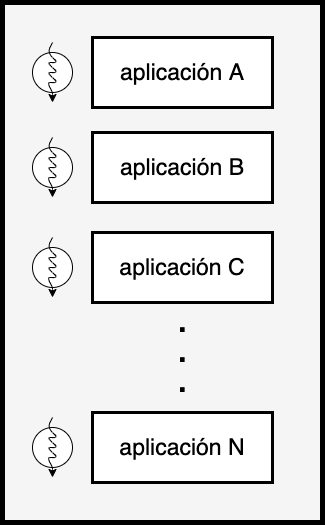
\includegraphics[scale=.3]{appN_h}
        \caption{Aplicaciones en ejecución concurrente en el CPU.}
        \label{fig:appN_h}
    \end{figure}

Al código de cada una de las aplicaciones se le debe añadir una serie de variables y parámetros para que el planificador pueda programar su ejecución. 
\newline

Se debe encapsular la llamada a la función kernel para que el planificador permita dar el orden de lanzamientos. Dentro de cada enclave se debe implementar una serie de variables y banderas para que el contexto pueda ser almacenado al alcanzar a cada punto preemptive. 
\newline

Es necesaria la definición de la estructura \textit{backup} específica del kernel, también se debe indicar la duración del quantum con \textit{quantum\_time}, una bandera de control para verificar si ya ha expirado el quantum y una bandera que indicará si ya se ha ejecutado completamente el kernel. Finalmente, el planificador dará permiso de que se ejecute el kernel con la variable de control \textit{continuar\_eje}.
\newline

Ahora bien, una vez que se han definido las variables de control, se debe implementar un ciclo que terminará hasta que el kernel sea completado. Dentro debemos inicializar \textit{quantum\_expirado} en \textbf{\textit{false}} para indicar que se tiene tiempo de ejecución. La bandera \textit{continuar\_eje} será modificada por el planificador para permitir la ejecución del kernel. Una vez que sea planificado para su ejecución, se lanzará el kernel  y se esperará el tiempo definido para el quantum. Terminado este tiempo, se cambiará el estado de \textit{quantum\_expirado} a \textit{\textbf{true}} y se sincronizarán todos los threads del kernel con \textit{cudaDeviceSynchronize()} para cerciorarnos de que se terminó la ejecución del grid.

Ahora debemos cambiar el estado de \textit{continuar\_eje} a \textbf{\textit{false}} para que la tarea permanezca suspendida hasta que el planificador permita una nueva ejecución. Finalmente, se pregunta si todos los blocks completaron su trabajo.

\lstinputlisting[style=CStyle, frame=single,label=lst:lanzamiento,  basicstyle=\ttfamily\footnotesize, caption=Algoritmo para lanzamiento del kernel en el lado del host.]{algorithms/lanza_kernel.c}

Para poder determinar si un kernel ha terminado completamente su procesamiento, nos auxiliamos de la función \textit{kc} (Algoritmo \ref{lst:funcionkc}). Simplemente se pasa como parámetro el arreglo \textit{estado} de la estructura \textit{backup} y se pregunta si el estado de todos los blocks es \textit{\textbf{TERMINADO}}, regresando \textbf{\textit{true}}.

\lstinputlisting[style=CStyle, frame=single,label=lst:funcionkc,  basicstyle=\ttfamily\footnotesize, caption=Función kernel completo.]{algorithms/funcion_kc.c}

\section{Planificador} \label{secc:planificador}

El módulo principal del framework es el del \textbf{Planificador} (ver figura \ref{fig:Planificador}) porque es aquí donde se realiza toda la calendarización de las tareas a ser ejecutadas en la GPU. Trabaja muy estrechamente con el módulo de la asignación de prioridades, el cual le da la pauta para poder elegir aquella tarea que tenga mayor relevancia en un momento determinado en el tiempo. 

\lstinputlisting[style=CStyle, frame=single,label=lst:Task,  basicstyle=\ttfamily\footnotesize, caption=Estructura task.]{algorithms/Task.c}

Para poder planificar un conjunto de tareas en la GPU, es necesario conocer las particularidades de la arquitectura del sistema embebido en el que se implementará el framework. Esto es especialmente necesario para que conozcamos el número máximo de threads que pueden estar en ejecución concurrentemente.

    \begin{figure}[!]
      \centering
        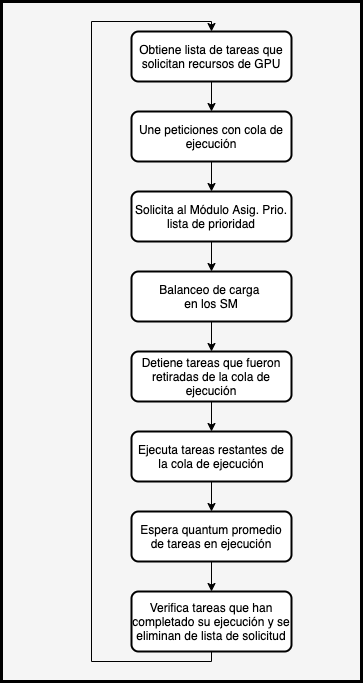
\includegraphics[scale=.6]{Planificador}
        \caption{Diagrama de flujo del planificador.}
        \label{fig:Planificador}
    \end{figure}

Cada uno de los kernels que soliciten recurso de cómputo en la tarjeta gráfica al planificador deberá ser mapeado a una estructura (algoritmo \ref{lst:Task}), la cual tendrá almacenados algunos de sus parámetros para ejecución, así como información relevante para la asignación de su prioridad en un instante de tiempo.
\newline

El algoritmo \ref{lst:planificador} muestra la manera en que deberá guiarse el programador para implementar el planificador, primero se obtiene la lista de tareas \textit{sol} que solicitan los recursos del GPU y las une con aquellas que ya se tenían en la cola de ejecución \textit{R}, esta cola contiene tanto las tareas que en una ejecución fueron beneficiadas de consumir recursos como aquellas que se mantienen en estado de ociosidad.

Se llama al módulo Asignación de Prioridad (ver sección \ref{secc:asigPrioridad}) para que devuelva la cola ordenada por prioridad \textit{r} (el orden depende del algoritmo de asignación de prioridades en tiempo real seleccionado).

La cola \textit{r} se envía a un balanceador de carga que ayudará a la maximización de la planificación de tareas ejecutables en un quantum. Posteriormente, detendrá la ejecución de aquellas que deban drenar su contexto en la iteración actual \textit{j} para darle lugar a una con mayor prioridad.
Se esperará un quantum \textit{x} (el estudio del quantum más apropiado queda fuera del contexto de esta tesis) y una vez alcanzado el plazo límite, se eliminarán de \textit{R} aquellas tareas que completaron su ejecución en la iteración \textit{j}. 

\lstinputlisting[style=CStyle, frame=single,label=lst:planificador,  basicstyle=\ttfamily\footnotesize, caption=Función planificador.]{algorithms/planificador.c}

\subsection{Balanceador de carga} \label{secc:balanceador}

Bajo suposición y asignación de una carga de trabajo, todas las tareas son preemptive debido a que por decisiones del hardware muchas veces no podrán asignarse aunque haya espacio para su ejecución.
\newline

Como se mencionó en el capítulo \ref{cha:TrabajoRelacionado} el orden de lanzamiento de los kernel a la GPU afecta la forma en que serán asignados a los SM. Por ejemplo, en el escenario a) (ver figura \ref{fig:Balanceo}. Primero se lanza \textbf{K1}, seguido de \textbf{K2} y al final \textbf{K3}, dando como resultado el desperdicio de recursos y que no sea posible ejecutar un kernel. Sin embargo, si se modifica este orden, se puede optimizar la asignación de tareas en las localidades, como lo vemos en el ejemplo b).
\newline

Por esta razón, se ideó un balanceador de carga que permitirá la maximización de la planificación de tareas ejecutables en un quantum.
\newline

        \begin{figure}[!]
      \centering
        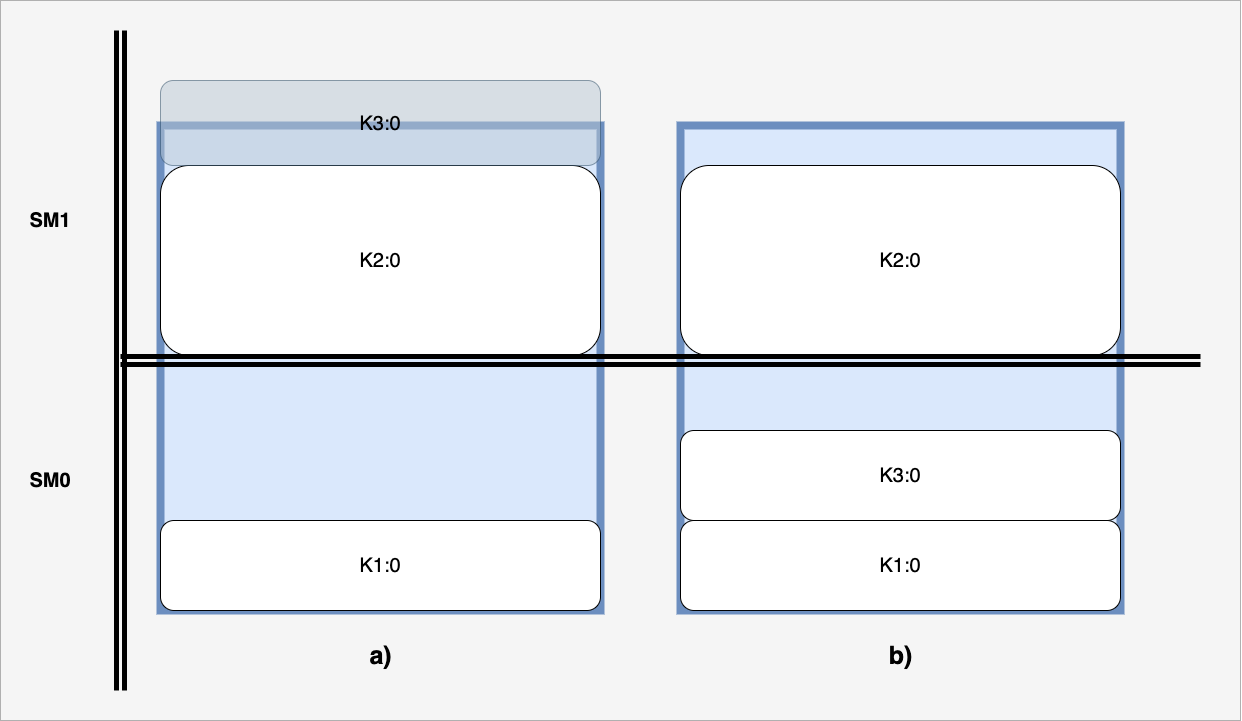
\includegraphics[scale=.24]{Balanceo}
        \caption{Diagrama de balanceo de carga de kernels en los SM.}
        \label{fig:Balanceo}
    \end{figure}
    
    Como se ha visto a lo largo de este trabajo, la asignación de recursos para la ejecución de kernels en la tarjeta gráfica no es algo trivial, por lo que fue necesario diseñar un balanceador de carga (ver figura \ref{fig:Balanceador}) que tomará en cuenta las características propias del sistema utilizado como caso de estudio.
    \newline
    
    Debido a que las tareas que serán ejecutadas sobre el sistema se presuponen embebidas, se considera que probablemente podrán ejecutarse al menos dos kernels en concurrente sobre la tarjeta, por lo que es imprescindible que ellas siempre tengan recursos suficientes para su ejecución. En caso de que la tarea de mayor prioridad absorba todos los recursos, no será necesario ejecutar la segunda tarea en ese quantum.
\newline

    \begin{figure}[!]
      \centering
        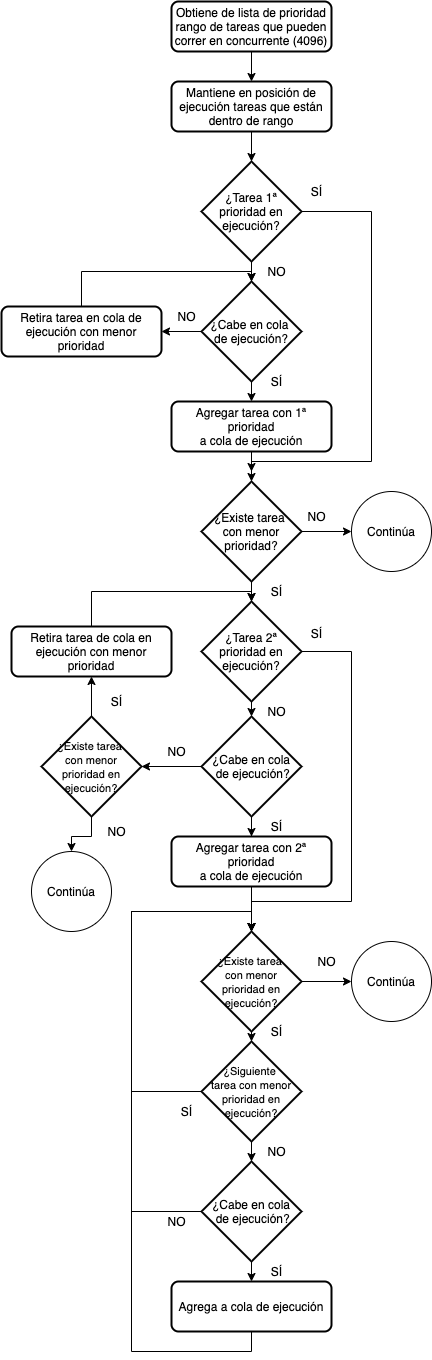
\includegraphics[scale=.41]{Balanceador}
        \caption{Diagrama de flujo del balanceador de carga.}
        \label{fig:Balanceador}
    \end{figure}

La lógica de asignación de tareas a los SM se basa en colocar la mayor cantidad posible de kernels en concurrente para que se puedan realizar más cálculos en menor tiempo.
\newline

    \begin{figure}[!]
      \centering
        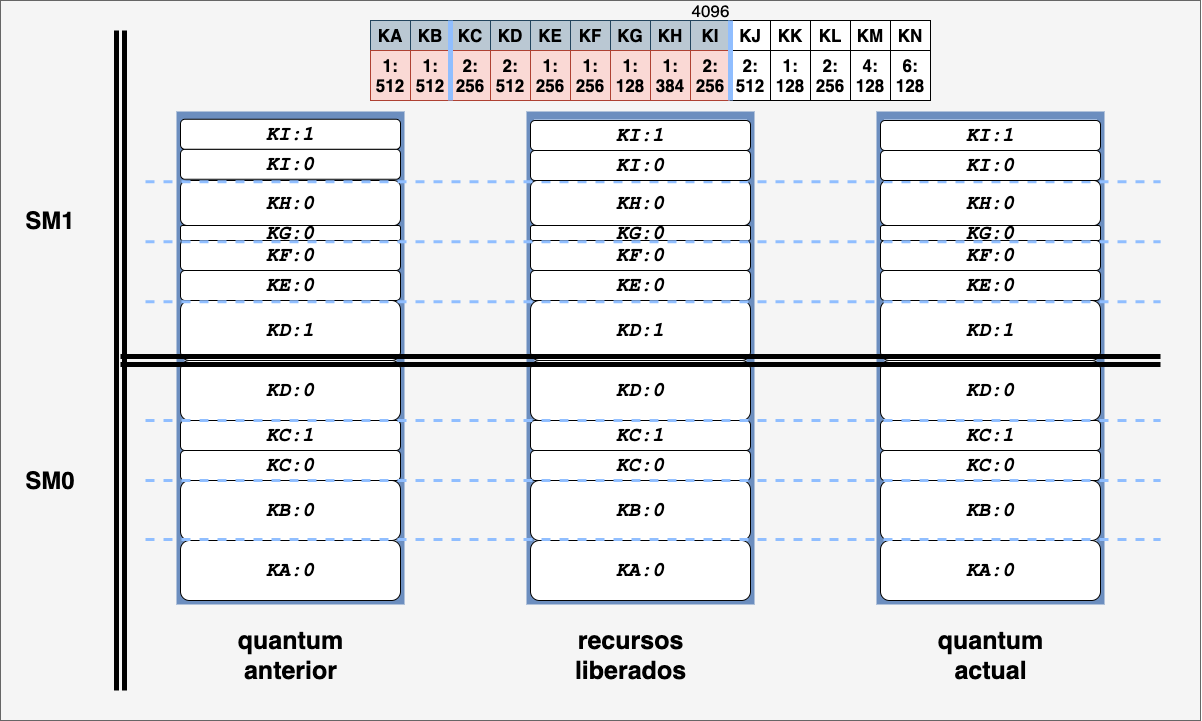
\includegraphics[scale=.26]{C1Balanceo}
        \caption{Caso I Kernels mantienen su prioridad en la siguiente iteración.}
        \label{fig:C1Balanceo}
    \end{figure}

A continuación se muestran algunos de los diversos escenarios en forma de casos de estudio que pueden aparecer al recurrir al balanceador de carga. Cada uno está representado en un diagrama, el cual posee en la parte superior la lista ordenada por prioridad (mayor a menor), cada tarea contiene el nombre del kernel así como el número de blocks que se requieren lanzar seguido del número de threads que los comprende. Se sombrean aquellas tareas que lograron ejecutarse en cada iteración, también se tiene una división en la lista. A la izquierda se comprenden las tareas que pudieran correr en concurrente en un punto en el tiempo de ejecución. A la derecha, aquellas que salen de dicha cuenta, justo en la última tarea de la primera mitad se tiene las suma de los threads que hipotéticamente pudieran ejecutarse en concurrente.
\newline

El Caso I (ver figura \ref{fig:C1Balanceo}), representa un escenario en donde la totalidad de las tareas que estaban ejecutándose en la iteración anterior a) vuelven a quedar en la posición de mayor prioridad en la lista en b), puesto que ninguna tarea tuvo que ser sacada de ejecución, se les dará oportunidad de un siguiente quantum sin necesidad de detenerse guardar su contexto y relanzarse.
    \newline
    
    \begin{figure}[!]
      \centering
        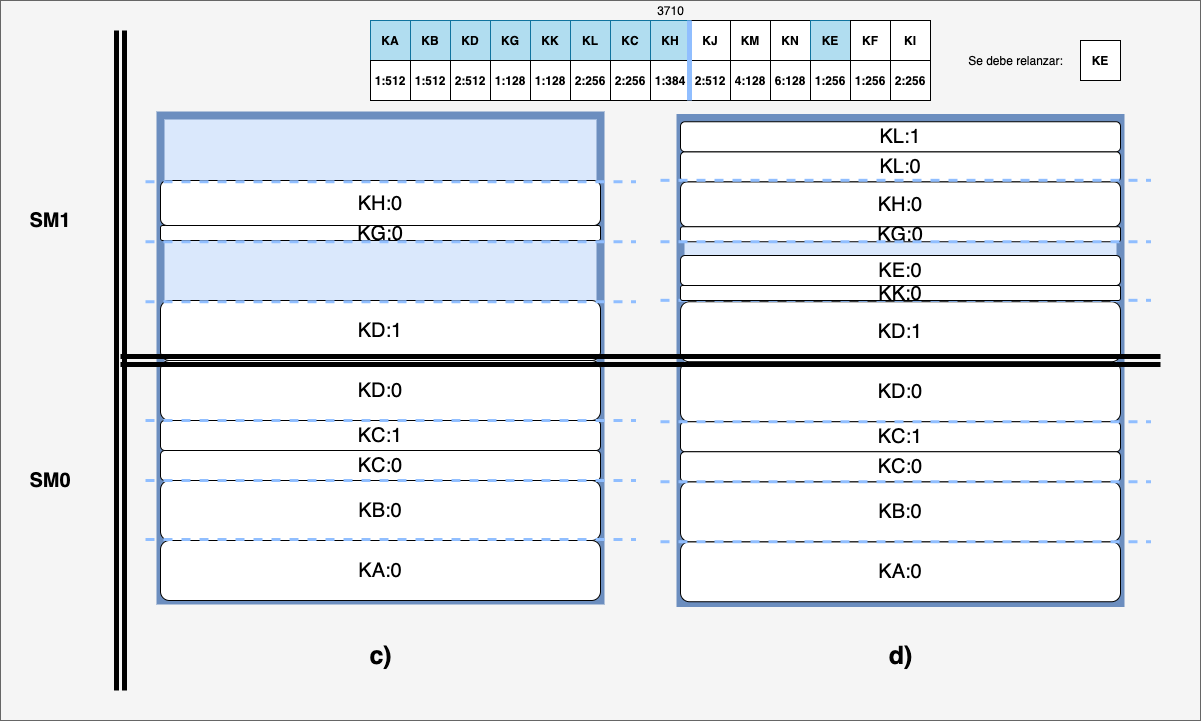
\includegraphics[scale=.26]{C2Balanceo}
        \caption{Caso II Kernels de baja prioridad deben relanzarse.}
        \label{fig:C2Balanceo}
    \end{figure}
    
    Una vez terminado el quantum de la iteración y recalculando la lista de prioridades observamos que se presenta el Caso II (ver figura \ref{fig:C2Balanceo}), donde algunas de las tareas ahora cambiaron el orden en la lista. Procedemos a calcular el rango de las tareas que pudieran correr en concurrente, y encontramos que la mayoría puede continuar en ejecución por que se encuentran del lado derecho. Aquellas que quedaron del lado derecho se deben sacar de la lista de ejecución y ser insertadas en la lista de paro de actividades para dar oportunidad de ejecución a aquellas que tienen mayor prioridad, para este caso serían los kernel \textbf{KE}, \textbf{KF} y \textbf{KI}. Luego, procedemos a agregar las del lado derecho por orden de prioridad, \textbf{Kk} y \textbf{KL}. 
    Una vez agregadas las tareas de mayor prioridad, se observa que aún queda espacio y se pregunta a las tareas de menor prioridad si sus características cumplen con los requisitos para que puedan ser ejecutadas en esa iteración, con ello concluimos que la tarea \textbf{KE} puede ingresar a ejecutarse.     
    \newline
    
    \begin{figure}[!]
      \centering
        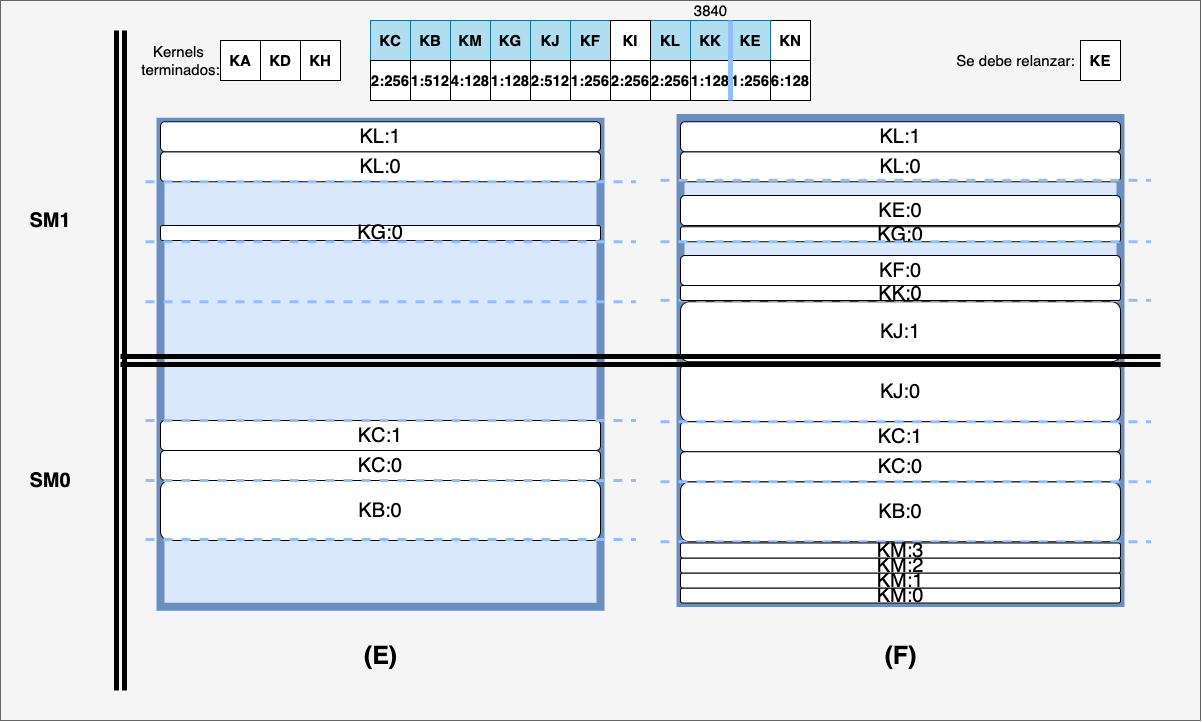
\includegraphics[scale=.26]{C3aBalanceo}
        \caption{Caso IIIa Kernels que completaron su ejecución.}
        \label{fig:C3aBalanceo}
    \end{figure}

    Después de terminada la iteración d), se encontró que las tareas \textbf{KA}, \textbf{KD} y \textbf{KH} han completado su ejecución, por lo que son eliminadas de la lista de peticiones. Por ello, la lista de prioridades para esta ejecución se modificó tanto en orden, como en longitud. Una vez calculado el rango de las posibles tareas en concurrente, encontramos que varias de ellas ya no existen, o bien, deben ser retiradas de ejecución para dar lugar a otras con mayor prioridad. En esta ocasión nos quedamos únicamente con \textbf{KB}, \textbf{KC}, \textbf{KG} y \textbf{KL}, y, procedemos a rellenar el espacio existente con las tareas según su orden de prioridad. 
    \newline
    
    \begin{figure}[!]
      \centering
        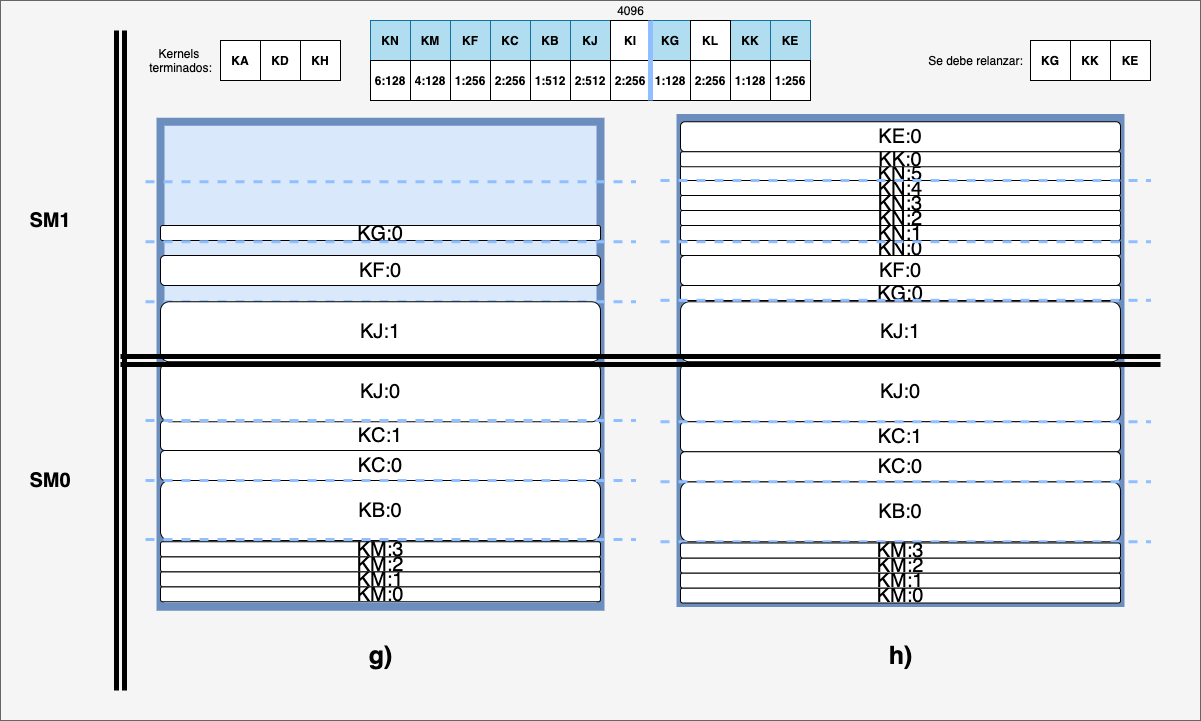
\includegraphics[scale=.26]{C3bBalanceo}
        \caption{Caso IIIb Kernels que completaron su ejecución.}
        \label{fig:C3bBalanceo}
    \end{figure}
    
    Pero en el Caso III (ver figura \ref{fig:C3aBalanceo}), debido a la forma en que están dispuestas las tareas, teóricamente la tarea \textbf{KI} debería poder ejecutarse porque hay suficientes threads para su ejecución, pero el hecho de que no estén contiguos imposibilita esta acción. 
    Por ello, se salta y se decide agregar tareas de menor prioridad, incluso \textbf{KE} que está del lado derecho de la lista de prioridad. Debido a que nuevamente tenía una baja prioridad y tuvo que ser quitada de ejecución, y, se le dió oportunidad de ejecutarse (sin importar si fuera en su misma ubicación) debe detener su ejecución, guardar su contexto y volver a ejecutarse.
\newline

    Siguiendo con el flujo del planificador, (ver figura \ref{fig:C3bBalanceo}) se vuelve a obtener una nueva lista de ejecución (nótese que del lado izquierdo se indica que se podrían utilizar los 4096 threads de los SM). Al momento de llenar la cola de ejecución por prioridad, aunque la tarea  \textbf{KI} nuevamente se queda fuera de ejecución, ahora ganamos recursos para 3 de menor prioridad \textbf{KG}, \textbf{KK} y \textbf{KE}. Como dichas tareas se encontraban en ejecución en la iteración pasada pero ahora son de baja prioridad, se deben detener para ser lanzadas nuevamente.
\newline

    \begin{figure}[!]
      \centering
        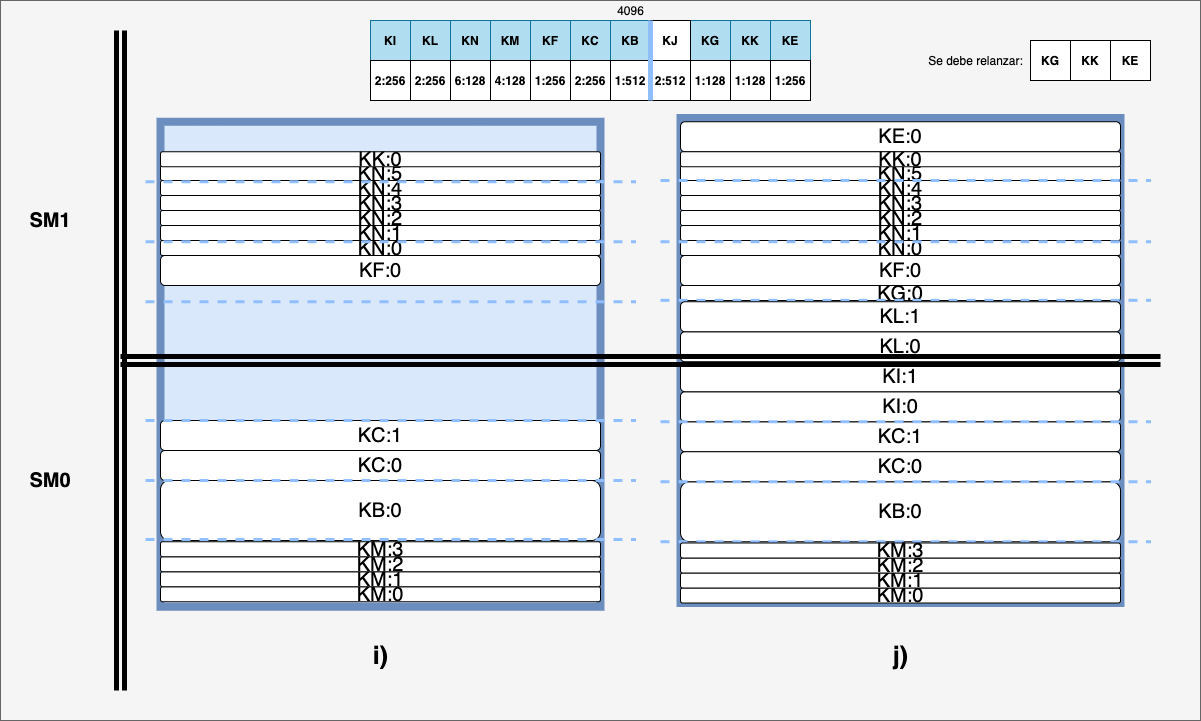
\includegraphics[scale=.26]{C4Balanceo}
        \caption{Caso IV Kernels muy grandes.}
        \label{fig:C4Balanceo}
    \end{figure}
    
    En el Caso IV (ver figura \ref{fig:C4Balanceo}) se tiene que la lista ordenada de prioridad del lado izquierdo contiene tareas que no ocupan por completo los recursos aportados por los SM, pero la primer tarea del lado derecho por sus características no puede ser ejecutada. 
    Por ello, no fue seleccionada en primer lugar, ya que es necesario empezar a llenar el espacio sobrante con las tareas de baja prioridad. En este caso, maximizamos la totalidad de los recursos de los SM y ejecutamos toda la lista de prioridad a excepción de la tarea \textbf{KJ}. Y nuevamente, como al inicio no estaban planeadas para su ejecución en esta iteración, se debe detener y relanzar a las tareas \textbf{KG}, \textbf{KK} y \textbf{KE}.
\newline

    \begin{figure}[!]
      \centering
        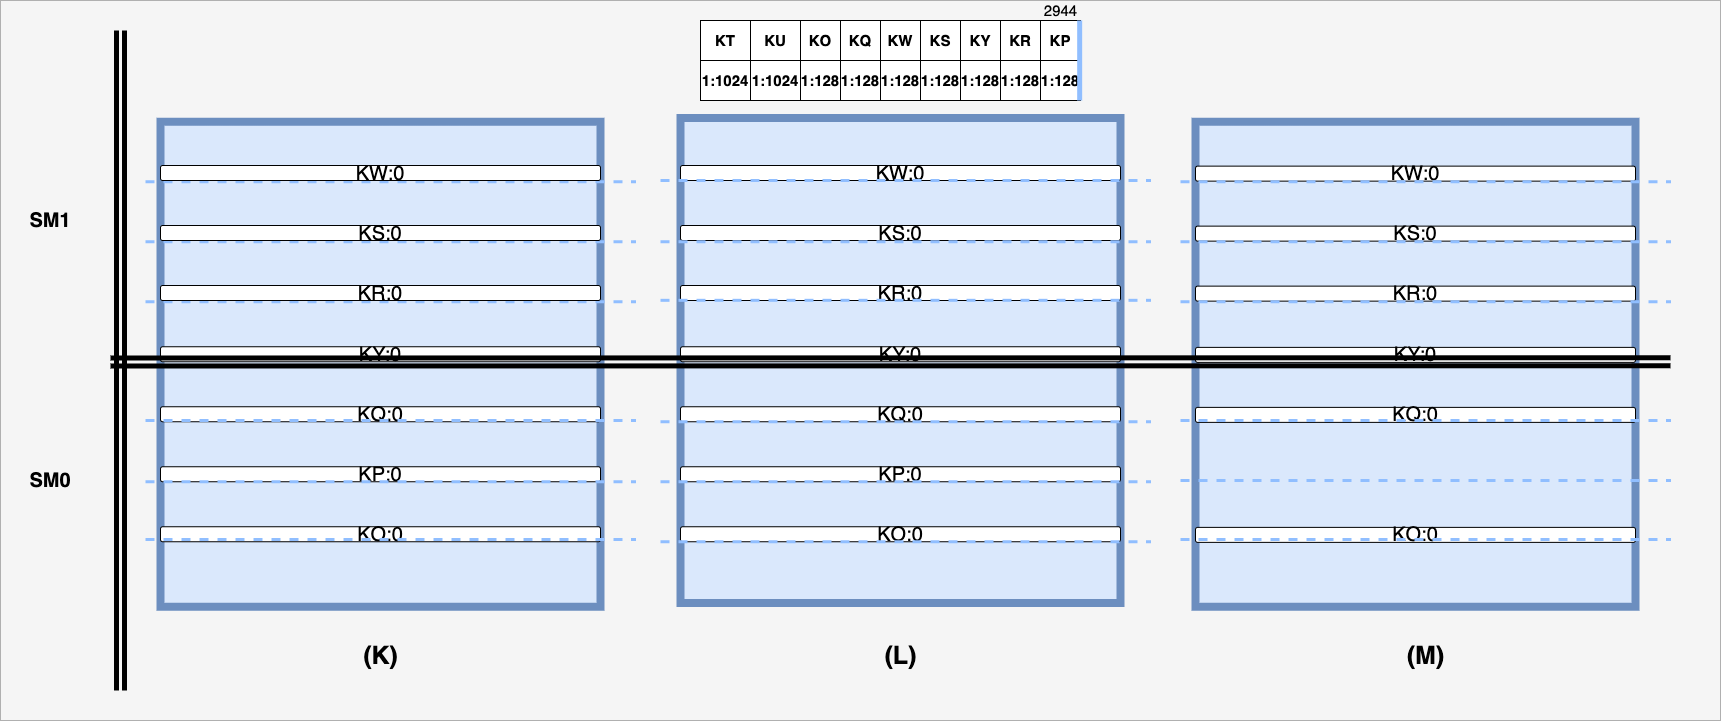
\includegraphics[scale=.25]{C5aBalanceo}
        \caption{Caso Va Kernels de mayor prioridad que no estaban en ejecución.}
        \label{fig:C5aBalanceo}
    \end{figure}
    
    \begin{figure}[!]
      \centering
        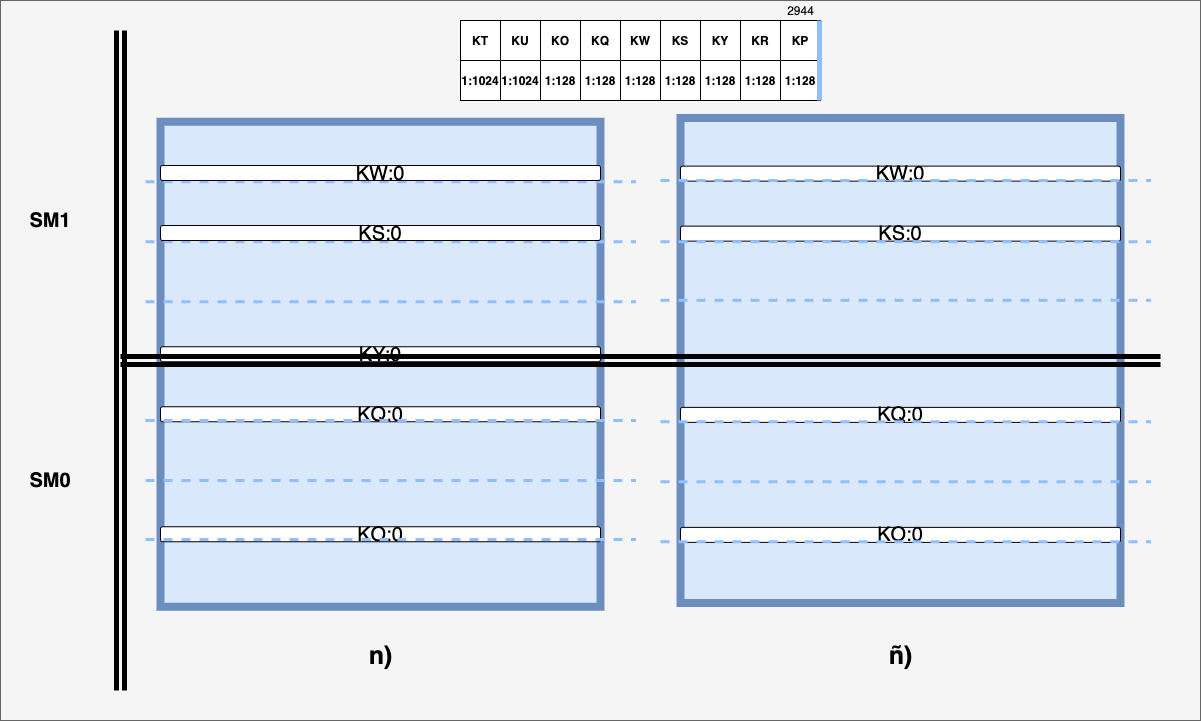
\includegraphics[scale=.26]{C5bBalanceo}
        \caption{Caso Vb Kernels de mayor prioridad que no estaban en ejecución.}
        \label{fig:C5bBalanceo}
    \end{figure}
    
    Después de diversas iteraciones del ciclo de vida del planificador, nos encontramos con el escenario k) (ver figura \ref{fig:C5aBalanceo}), donde tenemos que se encuentran en ejecución un cierto número de tareas esparcidas por los SM que utilizan solamente una fracción de sus recursos. Justo después de que se acaba el quantum de su iteración, se calcula nuevamente la lista de prioridad en l),y, ahora han aparecido dos tareas en la cabeza de la cola que solicitan recursos.
    Debido a que la de mayor prioridad no puede recibir recursos contiguos para su ejecución, se procede a sacar la tarea de menor prioridad actualmente en ejecución \textbf{KP}, y la de mayor prioridad pregunta nuevamente si ahora puede entrar en ejecución.
\newline

    Como no es posible que ingrese, se vuelve a quitar de ejecución la tarea con la menor prioridad (ver figura  \ref{fig:C5bBalanceo}), y así sucesivamente hasta que se reúnan las características que se requiere. Una vez liberado el espacio en ñ), se añade la tarea con la mayor prioridad en o), y se pregunta ahora por el espacio requerido por la tarea con la segunda mayor prioridad. Como nuevamente no se puede agregar a ejecución, se eliminan las tareas de menor prioridad hasta que sea posible colocarla.
\newline

    \begin{figure}[!]
      \centering
        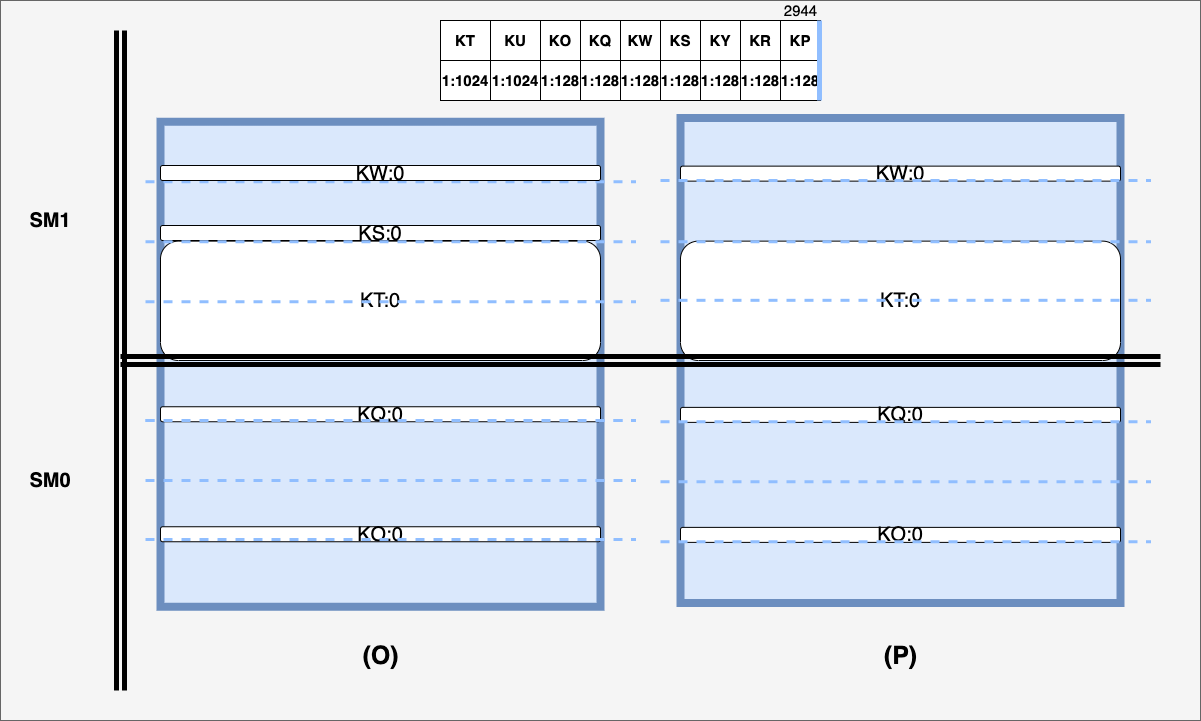
\includegraphics[scale=.26]{C5cBalanceo}
        \caption{Caso Vc Kernels de mayor prioridad que no estaban en ejecución.}
        \label{fig:C5cBalanceo}
    \end{figure}

    Una vez liberado el espacio contiguo necesario para la tarea \textbf{KT}(ver figura  \ref{fig:C5cBalanceo}), y así sucesivamente hasta que se reúnan las características que se requiere. Una vez liberado el espacio en ñ), se añade la tarea con la mayor prioridad en o), y se pregunta ahora por el espacio requerido por la tarea con la segunda mayor prioridad, como nuevamente no se puede agregar a ejecución, se eliminan las tareas de menor prioridad hasta que sea posible colocarla.
\newline
    
    \begin{figure}[!]
      \centering
        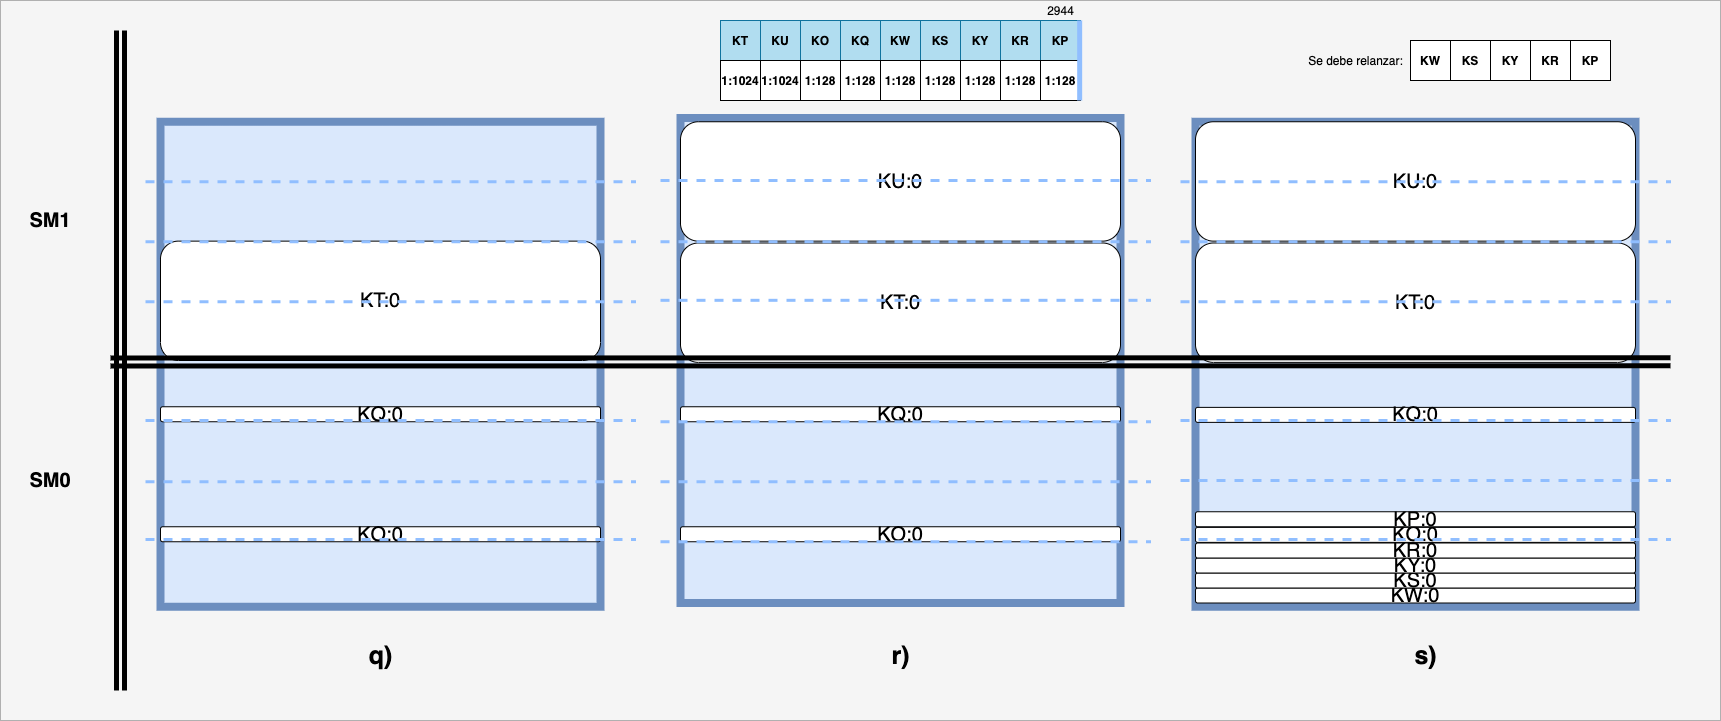
\includegraphics[scale=.26]{C5dBalanceo}
        \caption{Caso Vd Kernels de mayor prioridad que no estaban en ejecución.}
        \label{fig:C5dBalanceo}
    \end{figure}

   Liberado el espacio necesario (ver figura  \ref{fig:C5dBalanceo}), se procede a colocar la tarea \textbf{KU} y, posteriormente, se rellena el espacio con las tareas de la lista ordenada. Como se sacaron de ejecución las tareas \textbf{KW}, \textbf{KS}, \textbf{KY}, \textbf{KR} y \textbf{KP}, y después entraron nuevamente a la lista, es necesario relanzarlas.
\newline

    \begin{figure}[!]
      \centering
        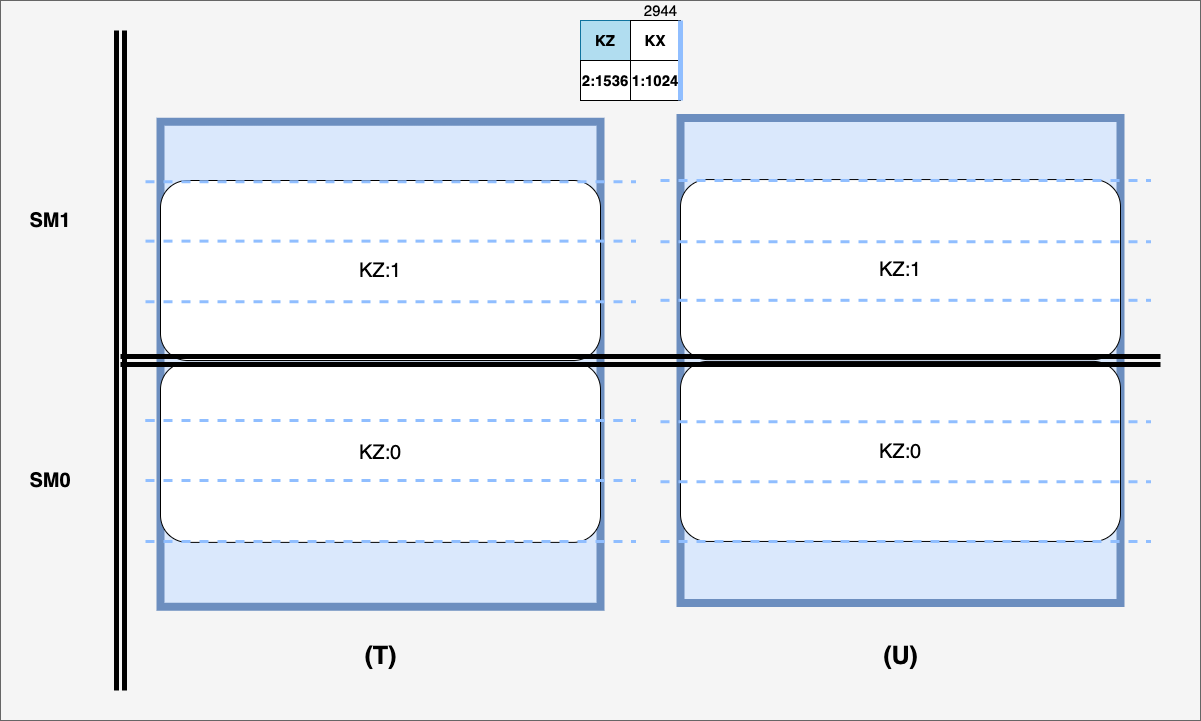
\includegraphics[scale=.26]{C6Balanceo}
        \caption{Caso VI.}
        \label{fig:C6Balanceo}
    \end{figure}
    En el Caso VI (ver figura  \ref{fig:C6Balanceo}), encontramos en q) que la tarea \textbf{KZ} ya se encontraba en ejecución, pero en la siguiente ejecución, se presentó la tarea \textbf{KW} con una prioridad menor, aunque teóricamente ambas tareas podrían ejecutarse concurrentemente, una tarea con menor prioridad no puede mover a una de mayor, por lo que en esta iteración únicamente se quedará en ejecución la tarea con la mayor prioridad.
    
\section{Asignación de prioridades} \label{secc:asigPrioridad}

Al tener como módulos separados tanto el planificador como la asignación de prioridades, nos da la flexibilidad de poder implementar diferentes algoritmos de tiempo real (ver \ref{sec:AlgoPlan}).
\newline

Para el diseño de este framework, se tomó como base el uso de algoritmos de asignación de prioridades en tiempo real de soporte monoprocesador, aunque no se descarta la posible implementación de aquellos que trabajan con multiprocesadores y subconjuntos de tareas. En este caso se asegura la ejecución de al menos dos tareas en concurrente en la tarjeta gráfica.
\newline

Dependiendo de las particularidades de cada algoritmo, se requerirá diferente información sobre la tarea a planificar, dichos parámetros podrán modificarse en la estructura (algoritmo \ref{lst:Task}) que mapea a las tareas.
\newline

Este módulo generará una lista de prioridad ordenando las tareas de mayor a menor, según sea el caso.
\newline

A cada iteración del planificador se asigna una prioridad a las tareas que actualmente están solicitando recursos de la GPU dependiendo de variables temporales. La planificación de las tareas del CPU pudieran ser manejadas por el sistema operativo o algún otro componente, pero su estudio está fuera del contexto de esta tesis.
\newline

El ejemplo de un posible algoritmo para la asignación de la prioridad de las tareas se muestra en el capítulo \ref{cha:Rendimiento}.